\documentclass{article}
\usepackage[utf8]{inputenc}
\usepackage[spanish]{babel}
\usepackage{listings}
\usepackage{graphicx}
\graphicspath{ {images/} }
\usepackage{cite}

\begin{document}

\begin{titlepage}
    \begin{center}
        \vspace*{1cm}
            
        \Huge
        \textbf{Nociones de la memoria de un computador.}
            
        \vspace{0.5cm}
        \LARGE
       
        \vspace{1.5cm}
            
        \textbf{Pedro Andrés Viloria Colón}
            
        \vfill
            
        \vspace{0.8cm}
            
        \Large
        Despartamento de Ingeniería Electrónica y Telecomunicaciones\\
        Universidad de Antioquia\\
        Medellín\\
        Septiembre de 2020
            
    \end{center}
\end{titlepage}

\tableofcontents

\section{Sección introductoria}
La memoria es fundamental en el desarrolo de aplicativos en el área infromatica. Conocer las capacidades gestión de memoria de nuestra maquina, nos ayuda  atomar las mejores decisionea la momento de programar.


El conocimiento básico de esta realidad, debe ser preocupación de todos los que desarrollan actividades relacionadas con este medio.

\section{Memoria del computador.} \label{contenido}
La memoria cumple un papel muy importante en el computador y su funcionamiento, ya que se
trata del dispositivo donde se almacena temporalmente toda la información con la que trabajan
los microprocesadores para procesarla y devolver los resultados que los usuarios requieren.
Se podría realizar la siguiente analogía; imaginen un empleado que debe realizar una serie de tareas contables. El cajón donde se guardan los documentos administrativos, podría considerarse equivalente a un disco duro; los documentos son equivalentes a los datos e información a procesar; el escritorio o mesa de trabajo donde se apilan dichos documentos
sería equivalente a la memoria del computador donde se almacena temporalmente la
información que se encuentra en procesamiento; mientras que la persona o su cerebro vendría
a ser como un procesador que realizará las distintas tareas:
    
 1) Primero se sacan del cajón (disco duro) los documentos administrativos y se los lleva a un escritorio (memoria) donde se apilan para poder trabajar. Se toma un primer documento de la pila para que el empleado (microprocesador) realice los cálculos necesarios, así como otras tareas y finalmente se ingresan las modificaciones o resultados de datos procesados en dicho documento. Se regresa dicho documento procesado a otra parte del escritorio (memoria) donde se colocarán los documentos procesados.
    
2) Luego se toma otro documento de la pila de documentos no procesados y se repiten los dos pasos anteriores. Eso se reitera una y otra vez hasta que todos los documentos hayan sido procesados.

3) Finalmente cuando se terminan de procesar todos los documentos, los cuales se encuentran apilados en la parte del escritorio (memoria) de documentos ya procesados, se toman y se vuelven a guardar en el cajón (disco duro) de almacenamiento de archivos. \cite{Desconocido}

\section{Tipos de memoria.} \label{contenido}
En un computador hay varios tipos de memoria, ordenados en jerarquías de velocidad y capacidad.

\begin{itemize}
    \item Memoria cache L1, L2 y L3.
    \item Memoria RAM.
    \item Memoria virtual.
    \item Disco duro. 
\end{itemize}
 

Cuanto más bajamos en la lista desde la memoria Cache hacia el disco duro, decrece la velocidad
de los distintos tipos de memoria y aumenta su capacidad.
Los microprocesadores actuales son muy rápidos y funcionan a miles de millones de ciclos por
segundo Ghz (Gigahertz), lo cual significa que pueden procesar miles de millones de bytes por
segundo. Por esta razón requieren de dispositivos de almacenamiento temporal de alta
velocidad que puedan seguirle el ritmo, de lo contrario se detendría para aguardar que la
información le llegue.
Sin embargo hay un pequeño problema, y es que la memoria que puede funcionar a la misma
velocidad del microprocesador es muy cara; y en grandes cantidades harían inalcanzable los
costos de un computador personal hogareña.
Pero los ingenieros encontraron una solución a este problema, utilizando el tipo de memoria
más veloz, Cache, en pequeñas cantidades, y la memoria RAM en mayores cantidades. Cada vez
que el microprocesador se da cuenta que un segmento de datos o información se utiliza de
manera reiterada, toma una copia de la RAM y la carga en la memoria Cache. Y a su vez de esta información la más utilizada la lleva a la Cache de nivel 1, o sea L1, que se encuentra dentro de
los mismos núcleos del microprocesador, funcionando a la misma velocidad de éstos. Los datos
que utiliza un poco menos los coloca en la memoria Cache L2, que también se encuentra dentro
de los núcleos, pero es un poco más lenta que la anterior, sin embargo puede tener mayor
capacidad, mientras que el resto de la información "cacheada" la coloca en la L3 que puede
llegar a tener como 12 Megabytes en promedio.
En el próximo nivel de jerarquía se encuentra la memoria principal del computador, la memoria
RAM, que a pesar de ser más lenta que la memoria Cache, es muchísimo más rápida que el disco
duro y se puede tener en grandes cantidades a un precio accesible; por lo que cuando se trabaja,
la mayor parte de la información se carga en ella y solamente aquellas pequeñas porciones que
se utilizan seguido van hacia la memoria Cache. De este tipo de memoria hablaremos más
adelante con mucho detalle ya que es la que más nos interesa en este artículo.
Después en el nivel de jerarquías le sigue la memoria virtual que no es otra cosa más que una
porción del disco duro dedicada exclusivamente a "sostener" temporalmente los pedazos de los
programas y datos en ejecución que se utilizan menos o que ocupan espacio innecesario en
algún momento determinado y es preferible colocarlos en una zona de reserva donde siempre
estarán listos para ser utilizados cuando se los requiera, pero que no ocuparán
innecesariamente los espacios limitados de la memoria.

Por lo general hacia 2012 era normal tener 4 Gigabytes de memoria RAM en el computador,
pero qué ocurriría si se comienzan a utilizar simultáneamente programas que requieren mucho
espacio, como por ejemplo un juego, mientras se está bajando una película para ver luego y el
siempre presente sistema operativo funcionando a todo momento (especialmente Windows
Vista que derrocha gracias a sus recursos y algunas fallas de programación mucho espacio de
memoria); la solución es reservar un espacio de memoria virtual en el disco duro (por ejemplo
en mi computador, que cuenta con 3 Gigabytes de memoria RAM, el sistema operativo Windows
7 me recomienda reservar 4 Gigabytes de memoria virtual). Con la memoria virtual, cada vez
que hay algún recurso de un programa que ocupa mucho volumen de la memoria RAM y todavía
no se está utilizando, se coloca hasta próximo aviso en la memoria virtual. De esta forma esa
parte disponible puede ser utilizada por otros recursos en uso.
La clave para un mejor rendimiento del computador y depender menos de la memoria virtual,
siempre es tener mayor cantidad de memoria RAM; de esta manera cuando se está trabajando
con muchos programas y tareas a la vez, solamente se puede percibir que se está utilizando la
memoria virtual cuando se pasa de un programa a otro ocurriendo una pequeñísima pausa de
hasta quizá 1 segundo, y nada más. Sin embargo si este no es el caso y se cuenta con poca
memoria RAM y el computador tiene que mover constantemente información entre la memoria
RAM y la memoria virtual del disco duro, el funcionamiento de la máquina se vuelve muy lento,
provocándose un efecto indeseado llamado hiperpaginación (thrashing en inglés). El término
proviene de páginas, ya que las porciones de la memoria RAM que se almacenan temporalmente
en la memoria virtual del disco duro se guardan en archivos temporales llamados archivos de
página, que en Windows tienen la extensión .SWP.
Es bueno dejar claro que la memoria virtual, simplemente sirve para "sostener" porciones de
un programa que no se está utilizando "todavía" pero que en cualquier momento sí se
utilizará; y que dado que el disco duro es mucho más lento que la memoria RAM no es bueno
depender mucho de ella; y lo mejor siempre es contar con la mayor cantidad posible de
memoria RAM.

El tamaño en bits de un Microprocesador indica cuánta información puede procesar o
manipular simultáneamente; por ejemplo un microprocesador de 32 bits puede procesar 4
bytes al mismo tiempo (ya que 32 bits equivalen a 4 bytes); mientras que un microprocesador
de 64 bits puede procesar o manipular 64 bits simultáneamente. Por otro lado la velocidad de
procesamiento por segundo de un microprocesador se mide en la cantidad de ciclos por
segundo que marca su reloj, o sea que si tenemos un microprocesador de 2 Ghz (Gigahertz) o
ciclos por segundo; cuenta con cuatro núcleos, y puede realizar tareas en cada "pulso" o ciclo
del reloj; si es de 64 bits (o sea que puede procesar 64 bits simultáneamente) puede procesar
potencialmente hasta 64 Gigabytes de información por segundo (2000 millones x 64 x 4 / 8).
Obviamente estos números no se dan en la realidad ya que tiene que traer y llevar esa cantidad
de información de y hacia la memoria RAM, la cual no puede trabajar a la misma velocidad del
microprocesador, de hecho es muchísimo más lenta, por lo que se tardan varios segundos en
enviar una cantidad tan grande de información, además que hacia el año 2012 la mayoría de los
computadores hogareñas no contaban con semejante cantidad de memoria RAM, lo más común
era tener unos 4 Gigabytes.

La velocidad de los módulos de memoria depende de la velocidad del bus, o sea las pistas del
circuito impreso de la placa madre por la que viaja la información de un dispositivo a otro, y
más concretamente de la velocidad del reloj del bus que une la memoria con el
microprocesador. Además depende de la cantidad de bits (pulsos eléctricos) que se transfieren
a la vez a través del bus que pueden ser 32 bits en máquinas más viejas o 64 bits en placas
madre de computadores comunes del año 2012
Así, si el módulo de memoria RAM se encuentra en una placa madre con un bus que funciona a
400 Mhz (400 millones de ciclos por segundo) y en cada ciclo del reloj se realiza una
transferencia de datos; y el bus es de 64 bits, o sea que se pueden transferir 64 bits
simultáneamente por las pistas del bus en cada ciclo; si multiplicamos 400.000.000 x 64 =
25.600.000.000 bits por segundo, y como cada byte está compuesto por 8 bits, si dividimos
25.600.000.000 / 8 = 3.200.000.000; esto significa que se pueden transferir teóricamente 3200
Megabytes por segundo. Obviamente estos números pueden variar por distintos motivos.
El principal motivo técnico que hace que estos números ideales de velocidad de transferencia
de datos no se den es la latencia. Cuando se transporta la información de la memoria RAM a su
microprocesador, también hay que tener en cuenta el tiempo en que tarda en leer dicha
información de la memoria. Por ejemplo cuando se quiere transmitir una serie de datos primero
hay que ir a buscarlos y si la lectura de dicha información puede durar 4 ciclos del reloj del bus,
ese tiempo deberá ser sumado a los valores de tiempo de transferencia; en otras palabras si el
reloj realiza 400.000.000 ciclos por segundo y en cada ciclo transporta 64 bits, esto significa
que requiere 0,0000000025 segundos (2,5 nanosegundos; o sea 2,5 mil millonésimas de
segundo) para transportar cada grupo de 64 bits, ya que cada ciclo del reloj del bus tiene una
duración de 2,5 nanosegundos. Pero supongamos que para llegar a leer los bits que luego serán
transferidos, como se mencionó antes, se necesita un tiempo de 4 ciclos del reloj del bus; por lo
que tardará 2,5 x 4 = 10 nanosegundos adicionales en leer los datos; más 2,5 para transferirlos,
entonces el tiempo total será de 12,5 nanosegundos; o sea 10 nanosegundos más que si la tarea
consistiera únicamente en transferir los datos de la memoria a su microprocesador.
Por eso para entender mejor cómo funciona la memoria principal del computador, a continuación analizaremos la memoria RAM.


 
\begin{figure}[h]
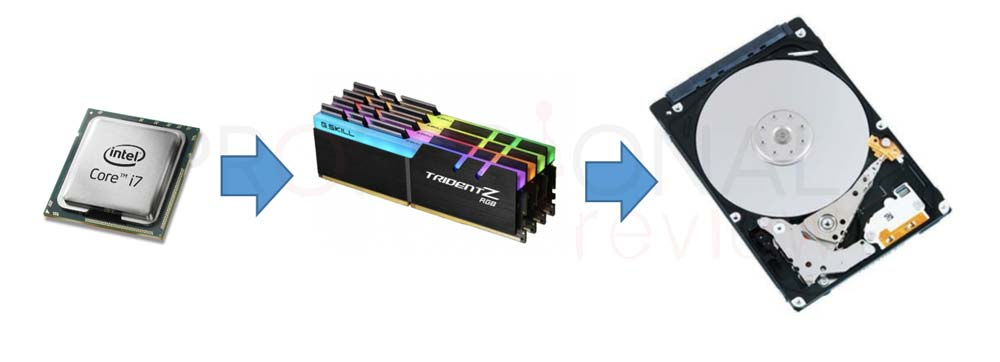
\includegraphics[width=5cm]{memorias.jpg}
 \cite{Red}
\centering
\caption{Memorias}
\label{fig:c}
\end{figure}

\section{¿Cómo funciona la memoria RAM?}\label{contenido} 
La memoria RAM es el tipo de memoria más importante del computador, su nombre representa
las siglas de Random Access Memory (Memoria de Acceso Aleatorio); la razón de dicho nombre
es porque la misma está dividida en celdas de memoria donde se almacenan cada uno de los
bits o pulsos eléctricos (que representan los 1 y 0) y a las cuales se puede acceder directamente
indistintamente de su posición o dirección. Lo opuesto a la memoria RAM sería el tipo de
memoria SAM o Serial Acces Memory (Memoria de acceso Serial) donde los datos se almacenan
en serie uno después del otro y los cuales solamente pueden ser accedidos secuencialmente,
como sucedía por ejemplo con un cassette, donde para llegar a un determinado punto de la cinta
hay que pasar primero por todos los puntos anteriores; mientras que en la memoria RAM los
datos pueden ser accedidos en cualquier orden.

Así como el microprocesador, un chip de memoria es un circuito integrado, compuesto por
millones de transistores y capacitores. La memoria RAM está dividida en celdas en donde se
almacenan temporalmente cada uno de los bits que componen los bytes de la información con
la que trabaja el microprocesador. Cada una de las celdas de la memoria que almacena un bit (1
o 0), se encuentra formada por un transistor y un capacitor. Mientras los capacitores sostienen
los bits de información, los transistores actúan como interruptores que permiten a su
controlador de memoria leer o modificar la información (los bits) que contienen cada una de
las celdas. A este tipo de memoria con celdas formadas por un capacitor y un transistor se la
denomina Dynamic Random Access Memory (Memoria de Acceso Aleatorio Dinámica) o por sus
siglas DRAM; a continuación les explicaré la razón por la que la memoria que utiliza ese tipo de
tecnología se denomina así.
Un capacitor es como una pequeña cubeta o balde que puede almacenar electrones; para
almacenar un bit equivalente a 1, se llena el capacitor con electrones; mientras que para
almacenar un bit igual a 0 se lo deja vacío. El único problema es que los capacitores son como
cubetas o baldes con orificios, así que si hacemos una analogía sería como llenarlos con agua la
cual se saldría por los orificios, por lo cual para mantenerlos llenos habría que echarles agua
constantemente, de lo contrario se vaciarían rápidamente. Los capacitores funcionan
exactamente igual, teniendo que ser recargados constantemente con electrones que
representan la información, antes de ser vaciados, cosa que ocurre en cuestión de pocos
milisegundos (para más información les recomiendo que lean Qué son los capacitores). 
Para mantener a los capacitores exactamente con la misma información de 1 (capacitores llenos de
electrones) y 0 (capacitores vacíos) sin que se modifiquen, el controlador de memoria tiene que
recargar los capacitores con 1 constantemente. Para hacer eso el controlador tiene que primero
leer la memoria y rellenar los capacitores aún cargados con electrones (o sea los que
representan a los bits 1) antes de que se descarguen. Esta operación de recarga ocurre
automáticamente varias veces por segundo.
Entonces como los capacitores se vacían rápidamente, si no fueran recargados toda la
información pasarían a ser bits iguales a 0, por ende haciéndola desaparecer. Este proceso de
recarga constante es de donde proviene el nombre de memoria dinámica RAM, ya que debe ser
dinámicamente recargada todo el tiempo para no perder la información que almacena. El punto
en contra de este tipo de tecnología es que hace que este tipo de memoria sea más lenta, el
punto a favor es que es económica y se puede tener en grandes cantidades a diferencia de la
memoria Cache.

\textbf{Las celdas de la memoria DRAM.}

La memoria está formada por celdas de bits distribuidas en una grilla bidimensional. Las celdas
de memoria (cada una compuesta por un capacitor y un transistor microscópicos) están
grabadas en láminas u obleas de silicio, distribuidas en una matriz de columnas
llamadas bitlines (líneas de bits) y filas llamadas wordlines (líneas de palabra), la intersección
de una columna y una fila determinan la dirección de una celda de memoria.
La memoria DRAM funciona enviando una señal o carga eléctrica RAS (Row Address Strobe o
Señal de Dirección de Fila) a la fila donde se encuentran las celdas cuyos transistores se van a
activar para poder permitir pasar a los electrones que se almacenarán en los capacitores de las
celdas. Una vez que la fila ha sido seleccionada mediante la señal RAS; para escribir los bits que
representan a los 1, se envían cargas eléctricas CAS (Column Address Strobe o Señal de
Dirección de Columna) a través de las correspondientes columnas para cargar con electrones a
los capacitores de las celdas que representan bits 1, mientras que las celdas que representan
bits 0 se mantienen vacías por lo que no se envían cargas a través de sus filas.
Por otro lado, para leer las celdas de la memoria de una fila, una vez seleccionada, mediante la
CAS, la columna que contiene la celda que se quiere leer, un detector de carga
llamado amplificador sensor (sense amplifier) determina el nivel de carga del capacitor de la
celda que se está leyendo; si detecta carga suficiente lo considera un bit 1 de lo contrario lo
considera un bit 0.
A su vez un controlador para mantener los capacitores de las celdas cargados, tiene que leer
cuáles son las celdas cargadas y luego las vuelve a cargar. Todo este proceso de lectura y
escritura ocurre en períodos de nanosegundos (mil millonésimas de segundo).
Las celdas de memoria (compuestas por un capacitor y un transistor) además dependen de
otros componentes para que la información pueda ser recibida y enviada correctamente por y
desde ellas. Algunas de las funciones que cumplen esos componentes son:
\begin{enumerate}
    \item Identificar cada fila y columna de una celda (RAS y CAS).
    \item Chequear la secuencia de recarga de celdas (contador); o sea que si se tienen que recargar una determinada cantidad de veces por segundo se van contando para saber cuándo hay que rellenarlas.
    \item Leer y reescribir la carga de una celda (amplificador sensor).
    \item Permitir o no permitir que una celda sea cargada (write enable - permiso de escritura).
\end{enumerate}


Otras funciones del controlador de memoria incluyen tareas como detección del tipo, velocidad
y cantidad de memoria; así como el chequeo de errores de escritura de datos, especialmente
durante el proceso de recargado de celdas, en que todo tiene que permanecer igual.


\textbf{La memoria estática (SRAM).} 

La memoria estática RAM (SRAM) utiliza una tecnología diferente a aquella de la memoria
DRAM. En la memoria estática cada celda de bit está compuesta por cuatro o seis transistores y
algunos circuitos; logrando que no sea necesario refrescar la información recargando las celdas
constantemente como sucede con la memoria dinámica. Eso hace que la memoria SRAM sea
más rápida que la DRAM, sin embargo por tener más partes o componentes en cada celda, las mismas ocupan mayor espacio que las celdas de memoria DRAM, obteniéndose menor cantidad
de bits de almacenamiento en un chip del mismo tamaño y por otro lado encareciendo los costos de las memorias por la mayor cantidad de partes.
Dado que la memoria SRAM es más rápida y costosa que la memoria DRAM, se la utiliza para la memoria caché del microprocesador.
\cite{Desconocido}

\section{Gestión de memoria en un computador.}\label{contenido} 

Se denomina gestión de memoria al acto de gestionar la memoria de un dispositivo informático. De forma simplificada se trata de proveer mecanismos para asignar secciones de memoria a los programas que las solicitan, y a la vez, liberar las secciones de memoria que ya no se utilizan para que estén disponibles para otros programas. 

La memoria es uno de los principales recursos de la computadora, la cual debe de administrarse con mucho cuidado. Aunque actualmente la mayoría de los sistemas de cómputo cuentan con una alta capacidad de memoria, de igual manera las aplicaciones actuales tienen también altos requerimientos de memoria, lo que sigue generando escasez de memoria en los sistemas multitarea y/o multiusuario.

La parte del sistema operativo que administra la memoria se llama administrador de memoria y su labor consiste en llevar un registro de las partes de memoria que se estén utilizando y aquellas que no, con el fin de asignar espacio en memoria a los procesos cuando éstos la necesiten y liberándola cuando terminen.

\textbf{Características.}

\textbf{Protección.}
La protección de memoria es un método para controlar el uso de memoria en una computadora, y es parte esencial de prácticamente todos los sistemas operativos modernos. El principal propósito de la protección de memoria es evitar que un proceso en un sistema operativo acceda a la memoria que no le ha sido asignada.

\textbf{Memoria compartida.}
Aunque la memoria utilizada por diferentes procesos suele estar protegida, algunos procesos puede que sí tengan que compartir información y, para ello, han de acceder la misma sección de memoria. La memoria compartida es una de las técnicas más rápidas para posibilitar la comunicación entre procesos.

\textbf{Organización lógica.}
Permiten que los programas se escriban como módulos compilables y ejecutables por separado.

\textbf{Organización física.}
La memoria suele dividirse en un almacenamiento primario de alta velocidad y uno secundario de menor velocidad.  La gestión de memoria del sistema operativo se ocupa de trasladar la información entre estos dos niveles de memoria.

\textbf {¿Por qué se necesita la gestión de memoria?}

\begin{enumerate}
    \item Para optimizar el espacio y poder cargar o intercambiar los programas que van hacer ejecutados del disco duro a la memoria principal.
    \item El administrador de memoria se encarga de llevar un registro de las partes de la memoria que están en uso y de las que no. Si detecta que hay una parte que ya no está en uso, la libera para poder asignarla a los procesos que la necesiten.
    \item  El administrador de memoria proporciona  protección y uso compartido, es decir, facilitar un espacio de memoria para cada proceso y controlar que ninguno de ellos trabaje en zonas de memoria que no le han sido asignados.
     \item Administrar el intercambio entre la memoria principal y el disco en los casos en los que la memoria principal no le pueda dar capacidad a todos los procesos que tienen necesidad de ella.
\cite{UM}
\end{enumerate}
\section{Rapidez de la memoria.}\label{contenido} 
Cuando se piensa en la capacidad de almacenamiento de un computador, lo primero que viene a la mente es el disco duro. Cuando se piensa en la velocidad del computador, en cambio, lo primero en que se piensa es en el procesador o en la memoria RAM. Es por esto que en el momento de hacer que un computador sea más rápido, lo primero que se suele hacer es ‘aumentar la RAM’. Sin embargo, el principal factor que influye en la velocidad de un computador es, paradójicamente, el disco duro. La razón está en la mecánica de funcionamiento. El disco duro de un computador es similar a un disco de acetato: un motor mecánico, en conjunto con un electroimán, mueven un cabezal rotativo sobre el que descansan los platos magnéticos en los que se graban los datos que se van a almacenar (sistema operativo, documentos, música, etc.). Estos datos son grabados y posteriormente leídos por una cabeza de lectura, también conocida como aguja. Es un mecanismo muy similar al que permite la reproducción de los discos de acetato. Y esto es justamente lo que hace que un computador se demore más o menos tiempo: en el momento de adquirir los datos requeridos, el cabezal debe dirigirse al sector del disco en el que están almacenados, y leerlos mientas el disco está rotando.

Es aquí donde se debe tener en cuenta, además de la capacidad de almacenamiento, las revoluciones por minuto (RPM) de un disco. Mientras mayor es el número de RPM, más rápido será el giro del disco y permitirá una lectura más rápida de dichos datos.Como alternativa a este proceso de lectura, es posible instalar a un computador un disco de estado sólido (o SSD, por las siglas en inglés de Solid State Drive). La principal diferencia está en la disposición de la memoria interna: en lugar de un plato giratorio, un SSD tiene varios módulos fijos de almacenamiento, similares a los que se encuentran en el interior de una memoria USB. Varias pruebas realizadas por el portal estadounidense web PCWorld mostraron una mejoría directa en el desempeño en computadores de diferentes marcas que fueron sometidos a pruebas de rendimiento en dos fases: primero, con sus discos duros originales y, posteriormente, con un cambio de la unidad de almacenamiento, conservando el mismo procesador, la misma cantidad de memoria RAM. Uno de los factores determinantes tras la prueba fue la aceleración del arranque y del acceso a los datos en dichos computadores. Miguel Orjuela, country Manager de Colombia y Ecuador de Kingston, asegura que la aplicación de este tipo de discos no se limita exclusivamente al uso de computadores. Varios centros de seguridad o de videograbación han optado por este tipo de almacenamiento para lograr un acceso más rápido a videos o datos guardados en sistemas consolidados de discos de estado sólido. Sin embargo, cada tipo de requerimiento tiene su propio tipo de almacenamiento, dependiendo de si es un uso corporativo, personal o de seguridad.
\cite{DISCO}


    
    
  
\section{Conclusión} \label{conclulsion}
Se ha podido comprender la importancia que juega la capacidad de memora y la gestión de esta, al momento de desarrollo de aplicativos. Conocer el equipo, en especial su memoria, ayuda a que se puedan realziar trabajos más concretos.
\bibliographystyle{IEEEtran}
\bibliography{references}

\end{document}
